%%%%%%%%%%%%%%%%%%%%%%%%%%%%%%%%%%%%%%%%%%%%%%%%%%%%%%%%%%%%%%%%%%% 
%                                                                 %
%                           INLEIDING                             %
%                                                                 %
%%%%%%%%%%%%%%%%%%%%%%%%%%%%%%%%%%%%%%%%%%%%%%%%%%%%%%%%%%%%%%%%%%% 


\chapter{Testen en Resultaten}  

In dit hoofdstuk worden de resultaten van het programma besproken. Vooraleer dit gedaan wordt zal er gekeken worden hoe de add-on moet worden geïnstalleerd en gebruikt. Dit zal worden gedaan aan de hand van een stappenplan.
\par
Er zal ook een vergelijking worden gedaan tussen een bestaand kristalvisualisatieprogramma en het programma als kristalvisualisatietool in Blender. Dit zal onder andere gedaan worden op basis van snelheid, gebruiksvriendelijkheid en uitbreidbaarheid.
\par
Er worden in dit hoofdstuk ook enkele valkuilen besproken die in de loop van dit onderzoek zijn opgedoken, en hoe deze worden opgelost. Sommige van deze valkuilen vormen echter grote problemen die in Blender moeilijk of niet kunnen worden vermeden. Er zal vermeld worden hoe deze problemen in dit onderzoek al dan niet zullen worden omzeild. Ten slotte zal er een blik worden geworpen op hoe het programma in de toekomst kan worden verbeterd en uitgebreid.
\par
Net zoals in hoofdstuk vier zal er voornamelijk gebruik worden gemaakt van de actieve schrijfwijze en de wetenschappelijke 'we'-vorm. 
\par 
In de eerste sectie staat een stappenplan dat het hele proces beschrijft dat moet gevolgd worden om met de add-on een kristal te tekenen in Blender. In de tweede sectie zullen resultaten van het programma worden beschreven. Hier worden onder andere enkele getekende kristallen weergegeven. In de derde sectie worden deze resultaten vergeleken met die van een ander kristalvisualisatieprogramma. 
\par
De vierde sectie zal de valkuilen bespreken waarmee dit onderzoek had te maken. In deze sectie worden ook enkele tekortkomingen van het programma gezien. In de vijfde, en voorlaatste, sectie van dit hoofdstuk wordt er gekeken naar wat de toekomst te bieden heeft voor het programma. Ten slotte zal er een conclusie gegeven worden waarin de belangrijkste punten van dit hoofdstuk nogmaals aan bod komen.   


\section{Een kristal tekenen met de add-on}
Deze sectie dient als een handleiding een gebruiker kan volgen om onze add-on te installeren in Blender en ze te gebruiken. Dit gaan we doen in de vorm van een stappenplan. 
\par
Dit is het stappenplan voor de installatie en het gebruik van de add-on op het besturingssysteem Windows. De add-on zou moeten werken op andere besturingssystemen maar de installatie van de add-on op deze gaan we niet bekijken. 

\subsection{Stap 1: Blender downloaden}
Als eerste moeten we Blender downloaden op ons syteem. Onze add-on is gemaakt voor versie 2.8x van Blender. In deze versie is er veel vernieuwd aan de Blender API waardoor de add-on niet achterwaarts compatibel is. Dit wil zeggen dat de add-on niet zal werken op oudere versies van Blender zonder de code aan te passen. In dit hoofdstuk spreken we, tenzij anders vermeld, altijd over de 2.8x versie van Blender .  
\par
Blender kan gedownload worden op de downloadpagina van hun offiële website:\url{https://builder.blender.org/download/}. Hier kiezen we het besturingssysteem en de bit-versie van ons systeem, en selecteren we de nieuwste versie van Blender, rode kader op Figuur[5.1].  Dit download het ZIP-bestand waarin de Blender installatie staat. Als de download voltooid is kunnen we het ZIP-bestand uitpakken op ons systeem. Dit creëert een map waarin de Blender installatie staat. In deze map vinden we het uitvoerbare bestand \textit{blender.exe}, waarmee we Blender opstarten. Dit is tevens ook de map waarin we de CifFile module in plaatsen, zie eerste sectie van hoofdstuk vier.      

\begin{figure}[h]
\begin{center}
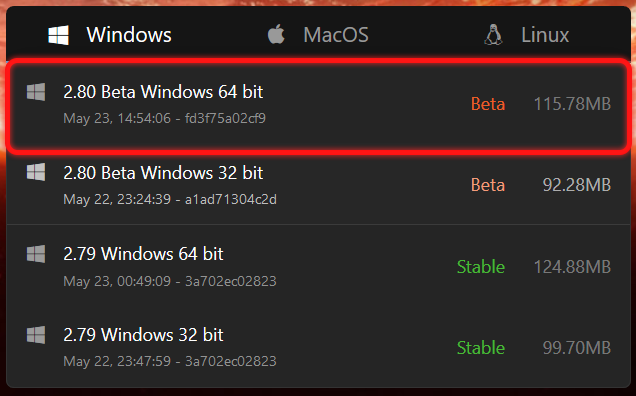
\includegraphics[scale=0.5]{b_download.png}
\caption{Overzicht van Blenderversies op downloadpagina van blender}
\end{center}
\end{figure}
 
\subsection{Stap 2: Externe programma's installeren}
Om de add-on te laten werken moeten we de OpenBabelGUI en de CifFile module van PyCIFRW op ons systeem installeren. We kunnen deze programma's downloaden op volgende webpagina's:

\begin{itemize}
\item OpenBabelGUI: \url{http://openbabel.org/wiki/Category:Installation}
\item PyCIFRW: \url{https://pypi.org/project/PyCifRW/#description}
\item CifFile map: \url{https://github.com/JarritB/Thesis/tree/master/} 
\end{itemize}   

Hoe we deze programma's werkende krijgen op ons systeem wordt uitgelegd in de eerste sectie van hoofdstuk vier. 
\par

\subsection{Stap 3: Add-on downloaden}
Op de GitHub pagina van dit onderzoek: \url{https://github.com/JarritB/Thesis/tree/master/blender-2.80.0-git.3c8c1841d72-windows64/2.80/scripts/addons} vinden we de map \textit{crystallographic\_interface}. Deze map bevat de code en dictionaries van onze add-on.
\par  
We downloaden de map en plaatsen deze in de \textit{addons} submap van de Blender installatie. (\textit{blender-2.80.0-git.3c8c1841d72-windows64 \textgreater \textgreater{} 2.80 \textgreater \textgreater{} scripts\textgreater \textgreater{} addons}) 

\subsection{Stap 4: Add-on activeren}
Om de add-on te activeren moeten we eerste Blender opstarten door \textit{blender.exe} uit te voeren. Vervolgens gaan we het venster met de \textit{user preferences} openen. Dit kunnen we doen op twee manieren: 
\begin{itemize}
\item In de linkerbovenhoek bij de optie \textit{Edit} (links op Figuur[5.2])
\item Zoekfunctie openen (F3-toets), en \textit{Show User Preferences} intypen (rechts op Figuur[5.2]) 
\end{itemize}     

\begin{figure}[h]
\begin{center}
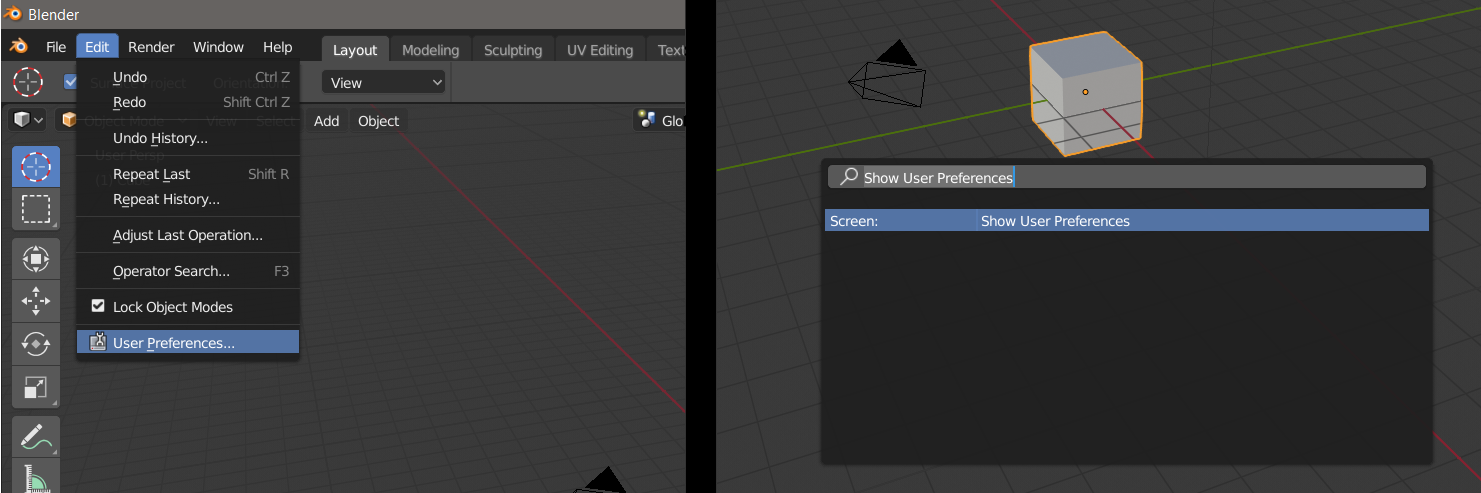
\includegraphics[width=\textwidth]{activ.png}
\caption{Openen van de \textit{User Preferences} via GUI(links) en Zoekfunctie(rechts)}
\end{center}
\end{figure}
 
Onder de tab \textit{add-ons} vinden we een lijst met add-ons die we kunnen gebruiken in Blender. Omdat we onze add-on in de map van Blender hebben geplaatst zou deze in de lijst moeten te vinden zijn onder de naam: \textit{Crystallography in Blender: Crystallographic Drawing Tool for Blender}. Om de add-on te activeren hoeven we enkel het selectievakje links van de naam aan te duiden. Als het vakje is aangevinkt is de add-on geactiveerd en klaar voor gebruik.

\subsection{Stap 5: Kristal tekenen met de add-on}
We kunnen de label van onze add-on zien onder het veld \textit{Tools} op het \textit{3D View} venster. Dit is het grote venster in het midden dat we zien wanneer we Blender opstarten. Het \textit{Tools} veld vinden we aan de linkerkant van dit venster, maar kan verborgen zijn. Met de T toets tonen en verbergen we tools veld. Bij het aanklikken van het \textit{CDTB} label zal ons paneel tevoorschijn komen. Als we osn in 'Edit Mode' bevinden zal het label niet getoont worden, door de Tab toets in te drukken geraken we terug in 'Object Mode', waar onze add-on zou moeten staan.  
\par   



\begin{table}[H]

\begin{center}
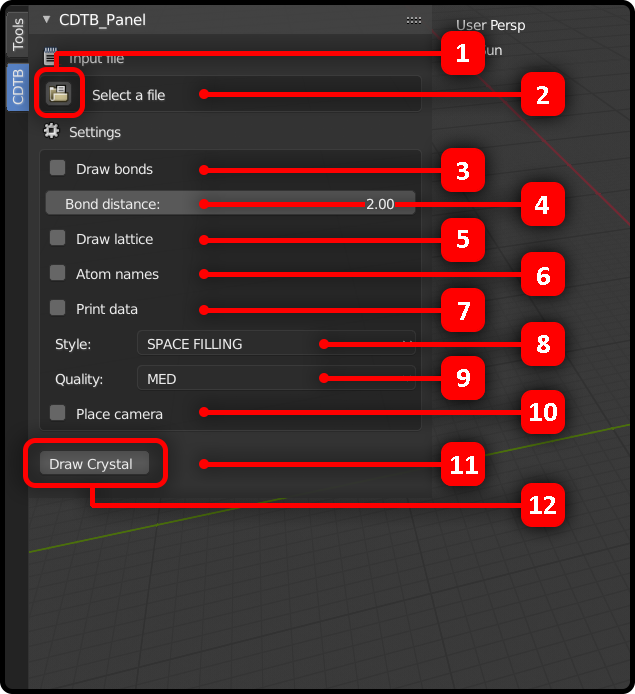
\includegraphics[scale=0.7]{numbers.png}
\end{center}

\begin{tabular}{|l|l|}
\hline
1  & Bij indrukken: opent een bestandsbrowser waar het CIF-bestand kan geselecteerd worden                                                                                                                                                                                \\ \hline
2  & Toont het geselecteerde CIF-bestand                                                                                                                                                                                                                                  \\ \hline
3  & Als aangeduid: tekent bindingen tussen de atomen                                                                                                                                                                                                                     \\ \hline
4  & Getal: bepaalt maximale afstand waartussen twee atomen worden gebonden                                                                                                                                                                                               \\ \hline
5  & Als aangeduid: tekent omkadering van de eenheidscel                                                                                                                                                                                                                  \\ \hline
6  & Als aangeduid: toont namen van de atomen op de tekening                                                                                                                                                                                                              \\ \hline
7  & Als aangeduid: drukt de kristalinformatie af in de Blender terminal                                                                                                                                                                                                  \\ \hline
8  & \begin{tabular}[c]{@{}l@{}}Keuzelijst: tekent kristal in gekozen stijl \\ \qquad STICK: toont enkel bindingen; \\ \qquad BALL AND STICK: toont verkleinde atomen, bindingen zichtbaar;\\ \qquad SPACE FILLING: toont atomen op ware grootte, bindingen meestan niet zichtbaar\end{tabular} \\ \hline
9  & Keuzelijst: bepaalt kwaliteit van de vormen, hogere kwaliteit verhoogt tekenduur                                                                                                                                                                                     \\ \hline
10 & Als aangeduid: plaats een camera en belichting, voor het renderen(F12) van het kristal                                                                                                                                                                               \\ \hline
11 & Bij indrukken: visualiseert het CIF-bestand                                                                                                                                                                                                                          \\ \hline
12 & Toont opmerkingen aan de gebruiker                                                                                                                                                                                                                                   \\ \hline
\end{tabular}
\caption{Overzicht van de functionaliteiten van de add-on}
\end{table}

Om een kristal te tekenen moeten we eerst een CIF-bestand selecteren. Dit doen we door met het icoon naast "Select a file" een bestandsbrowser te openen en ons CIF-bestand te selecteren. Dan hebben we de mogelijkheid om een aantal tekenvoorkeuren aan te passen, in Tabel[5.1] worden deze uitgelegd. Als we de voorkeuren hebben aangepast hoeven we enkel nog op de \textit{Draw Crystal} knop te klikken, en te wachten tot het kristal getekend is. Dit duurt, afhankelijk van de gekozen tekenopties en de grootte van het kristal, enkele seconden tot enkele minuten.
\par
  
\section{Resultaten}


Blender 2.80 is op het moment van dit onderzoek nog een beta versie, dit wil zeggen dat de versie instabiel zou kunnen zijn. Deze instabiliteit heeft echter geen problemen 
   